\documentclass{standalone}
\usepackage{tikz}
\usepackage{xinttools}

\usetikzlibrary{calc,math}


\begin{document}

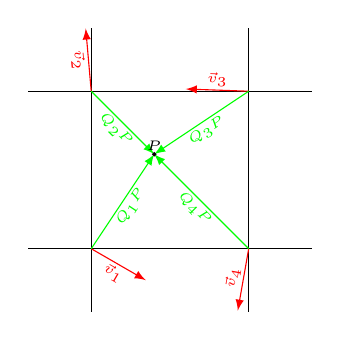
\begin{tikzpicture}[scale=2]
  \coordinate (P) at (0.4, 0.6);

  \draw (-0.4,-0.4) grid (1.4,1.4);

  \draw[-latex,red] (0,0) -- ++(-30:0.4) node[below,inner sep=1pt,font=\tiny,midway,sloped] {$\vec v_1$};
  \draw[-latex,red] (0,1) -- ++(95:0.4) node[below,inner sep=1pt,font=\tiny,midway,sloped] {$\vec v_2$};
  \draw[-latex,red] (1,1) -- ++(178:0.4) node[above,inner sep=1pt,font=\tiny,midway,sloped] {$\vec v_3$};
  \draw[-latex,red] (1,0) -- ++(-100:0.4) node[above,inner sep=1pt,font=\tiny,midway,sloped] {$\vec v_4$};

  \draw[latex-,green] (P) -- (0,0) node[below,inner sep=1pt,font=\tiny,midway,sloped] {$Q_1P$};
  \draw[latex-,green] (P) -- (0,1) node[below,inner sep=1pt,font=\tiny,midway,sloped] {$Q_2P$};
  \draw[latex-,green] (P) -- (1,1) node[below,inner sep=1pt,font=\tiny,midway,sloped] {$Q_3P$};
  \draw[latex-,green] (P) -- (1,0) node[below,inner sep=1pt,font=\tiny,midway,sloped] {$Q_4P$};

  \draw[fill=black] (P) circle [radius=0.01cm] node[above,font=\tiny,inner sep=1pt] {$P$};
\end{tikzpicture}

\end{document}
